\chapter{连通度和匹配}
  \begin{Def}
    图$G$的{\bfseries 顶点连通度}是指为了产生一个不连通图或平凡图所需要从$G$中去掉的最少顶点数目, 记为$\kappa (G)$。
  \end{Def}
  \centering
  \begin{minipage}{0.33\linewidth}
    
      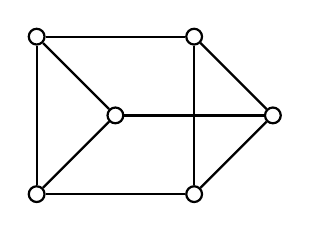
\begin{tikzpicture}[auto,
    specification/.style ={circle, draw, thick, inner sep = 0pt, minimum size=2mm}]
   \node[specification] (A)  at (0,-1)  {};
   \node[specification] (B)  at (0,1)  {};
   \node[specification] (C)  at (1,0)  {};
   \node[specification] (D) at (2,-1)  {};
   \node[specification] (E)  at (2,1)  {};
   \node[specification] (F)  at (3,0)  {};
   
   
   \draw[thick] (A) to  (B);
   \draw[thick] (B) to  (C);
   \draw[thick] (C) to  (A);
   
   \draw[thick] (D) to  (E);
   \draw[thick] (E) to  (F);
   \draw[thick] (F) to  (D);
   
   \draw[thick] (A) to  (D);
   \draw[thick] (B) to  (E);
   \draw[thick] (C) to  (F);
 \end{tikzpicture}  \end{minipage}
 \begin{minipage}{0.33\linewidth}
  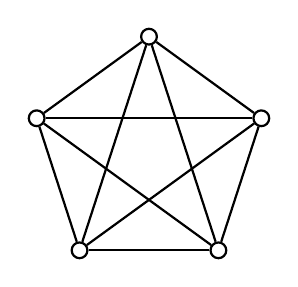
\begin{tikzpicture}[auto,
    specification/.style ={circle, draw, thick, inner sep = 0pt, minimum size=2mm}]
   \node[specification] (A)  at (18:1.5cm)  {};
   \node[specification] (B)  at (90:1.5cm)  {};
   \node[specification] (C)  at (162:1.5cm)  {};
   \node[specification] (D) at (234:1.5cm)  {};
   \node[specification] (E)  at (306:1.5cm)  {};
   
   \draw[thick] (A) to  (B);
   \draw[thick] (B) to  (C);
   \draw[thick] (C) to  (D);
   \draw[thick] (D) to  (E);
   \draw[thick] (E) to  (A);

   \draw[thick] (A) to  (C);
   \draw[thick] (A) to  (D);
   \draw[thick] (B) to  (D);
   \draw[thick] (B) to  (E);
   \draw[thick] (C) to  (E);

 \end{tikzpicture} \end{minipage}
\hspace{0.5cm}
 \begin{minipage}[c]{0.2\linewidth}
    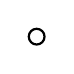
\begin{tikzpicture}[auto,
    specification/.style ={circle, draw, thick, inner sep = 0pt, minimum size=2mm}]
   \node[specification] (A)  at (0,0)  {};
 \end{tikzpicture}   
 \end{minipage}

  \begin{Def}
    图$G$的{\bfseries 边连通度}是指为了产生一个不连通图或平凡图所需要从$G$中去掉的最少边的数目, 记为$\lambda (G)$。
  \end{Def}
  \centering
  \begin{minipage}[c]{0.33\linewidth}
      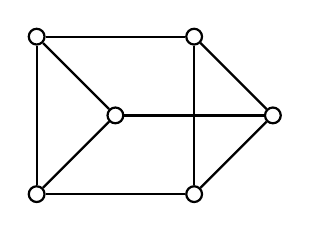
\begin{tikzpicture}[auto,
    specification/.style ={circle, draw, thick, inner sep = 0pt, minimum size=2mm}]
   \node[specification] (A)  at (0,-1)  {};
   \node[specification] (B)  at (0,1)  {};
   \node[specification] (C)  at (1,0)  {};
   \node[specification] (D) at (2,-1)  {};
   \node[specification] (E)  at (2,1)  {};
   \node[specification] (F)  at (3,0)  {};
   
   
   \draw[thick] (A) to  (B);
   \draw[thick] (B) to  (C);
   \draw[thick] (C) to  (A);
   
   \draw[thick] (D) to  (E);
   \draw[thick] (E) to  (F);
   \draw[thick] (F) to  (D);
   
   \draw[thick] (A) to  (D);
   \draw[thick] (B) to  (E);
   \draw[thick] (C) to  (F);
 \end{tikzpicture}    
  \end{minipage}
  \begin{minipage}[c]{0.33\linewidth}
   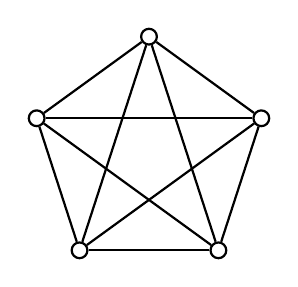
\begin{tikzpicture}[auto,
    specification/.style ={circle, draw, thick, inner sep = 0pt, minimum size=2mm}]
   \node[specification] (A)  at (18:1.5cm)  {};
   \node[specification] (B)  at (90:1.5cm)  {};
   \node[specification] (C)  at (162:1.5cm)  {};
   \node[specification] (D) at (234:1.5cm)  {};
   \node[specification] (E)  at (306:1.5cm)  {};
   
   \draw[thick] (A) to  (B);
   \draw[thick] (B) to  (C);
   \draw[thick] (C) to  (D);
   \draw[thick] (D) to  (E);
   \draw[thick] (E) to  (A);

   \draw[thick] (A) to  (C);
   \draw[thick] (A) to  (D);
   \draw[thick] (B) to  (D);
   \draw[thick] (B) to  (E);
   \draw[thick] (C) to  (E);
 \end{tikzpicture}   
 \end{minipage}\hspace{0.5cm}
 \begin{minipage}[c]{0.2\linewidth}
    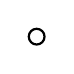
\begin{tikzpicture}[auto,
    specification/.style ={circle, draw, thick, inner sep = 0pt, minimum size=2mm}]
   \node[specification] (A)  at (0,0)  {};
 \end{tikzpicture}   
 \end{minipage}

  \begin{Thm}
    对任一图$G$,有 $\kappa (G) \leq \lambda (G) \leq \delta (G)$。
  \end{Thm}
  \begin{proof}[证明]
    先证$\lambda (G) \leq \delta (G)$。如果$\delta(G) = 0$,则$G$不连通或者为平凡图,此时$\lambda(G) = 0$,$\lambda(G)\leq \delta(G)$成立。如果$\delta(G)>0$,不妨设$\deg v = \delta(G)$,从$G$中去掉与$v$关联的$\delta(G)$条边之后,得到的图中$v$为孤立顶点,所以$\lambda(G) \leq \delta(G)$。因此,对任意的图$G$,$\lambda(G)\leq \delta(G)$。

    接下来证明$\kappa (G) \leq \lambda (G)$。如果$G$不连通或者为平凡图,则$\kappa(G)=\lambda(G)=0$。如果$G$是连通的且有一座桥$x$,则$\lambda(G)=1$。因为在这种情况下$G$或者有一个割点关联于$x$或者$G$为$K_2$,所以$\kappa(G)=1$。最后假定$\lambda(G)\geq 2$,则$G$中有$\lambda(G)$条边,移去它们后所得到的图不连通。显然,移去这些边中的$\lambda(G)-1$条边后得到一个图,它有一条桥$x=uv$。对于这$\lambda(G)-1$条边中每一条,选取一个关联于它但与$u$和$v$都不同的顶点。移去这些顶点之后就移去了这$\lambda(G)-1$条边。如果这样产生的图是不连通的,则$\kappa(G) < \lambda(G)$。否则,$x$是这样产生的图的一条桥,从而移去$u$或$v$就产生了一个不连通图或平凡图。所以,在任何情况下,$\kappa(G) \leq \lambda(G)$。
  \end{proof}

    \begin{Thm}
    对任何整数$a,b,c$, $0 < a \leq b \leq c$, 存在一个图$G$使得\[\kappa (G)
      = a, \lambda (G) = b, \delta (G) = c\]
  \end{Thm}

    \begin{Thm}
    设$G=(V,E)$有$p$个顶点且$\delta(G) \geq [ \frac{p}{2} ]$,则$\lambda(G) = \delta(G)$。
  \end{Thm}
  \begin{proof}[证明]
     $\lambda(G) \leq \delta(G)$显然成立, 只需要证明$\lambda(G) \geq \delta(G)$。

     

    因为$\delta(G) \geq [\frac{p}{2}]$,所以$G$是连通的。 如果$G$为平凡图, 则$\lambda (G) = \delta(G) = 0$。如果$G$不是平凡图,则$\lambda(G) > 0$,从而存在$V$的真子集$A$使得$G$中联结$A$中的一个顶点与$V\setminus A$中的一个顶点的边恰有$\lambda(G)$条。 所有这些边的集合记为$F$。

   由$|A| + |V\setminus A| = p$知必有$|A| \leq [\frac{p}{2}]$或者$|V\setminus A| \leq [\frac{p}{2}]$。 不妨设$|A| \leq [\frac{p}{2}]$。  由于$\delta(G) \geq [\frac{p}{2}]$,$A$中的每个顶点至少与$V\setminus A$中的一个顶点邻接。 否则,如果$A$中的某个顶点$u$只与$A$中的顶点邻接,则$\deg u \leq |A|-1 \leq [\frac{p}{2}] - 1 < \delta(G)$,矛盾。 
    设$v$为$A$中的任一顶点, $v$与$V\setminus A$中的$x$个顶点邻接,与$A$中的$y$个顶点邻接,则$\deg v = x + y$。  $v$与$V\setminus A$中的$x$个顶点邻接,所对应的边的集合记为$F_1$,则$F_1 \subseteq F$;
    $v$与$A$中的$y$个顶点邻接,而这$y$个顶点中的每个顶点都至少与$V\setminus A$中的一个顶点邻接,所对应的边的集合记为$F_2$,则$F_2 \subseteq F$ 并且$F_1 \cap F_2 = \phi$,从而
    \[\lambda(G) \geq |F_1| + |F_2| = x + y = \deg v \geq  \delta(G)\]
  \end{proof}

    \begin{Def}
    设$G$为一个图,如果$\kappa (G) \geq n$,则称$G$为{\bfseries $n$-顶点连通}的,简称$n$-连通;如果$\lambda (G) \geq n$,则称$G$为{\bfseries $n$-边连通}的。
  \end{Def}

    \begin{Thm}
    设$G=(V,E)$为有$p$个顶点的图,$p \geq 3$,则$G$为2-连通的,当且仅当$G$的任意两个不同的顶点在$G$的同一个圈上。
  \end{Thm}
  \begin{Def}
    设$u$与$v$为图$G$中的两个不同的顶点。两条联结$u$与$v$的路,如果除了$u$与$v$外没有公共顶点,则称这两条路为联结$u$与$v$的{\bfseries 不相交路};如果联结$u$与$v$的两条路上没有公共边,则称这两条路为联结$u$与$v$的{\bfseries 边不相交路}。
  \end{Def}
  \begin{Thm}
    图$G$为$n-$连通的当且仅当每一对不同顶点间至少有$n$条不相交路。
  \end{Thm}
  \begin{Thm}
    图$G$为$n-$边连通的当且仅当$G$的任一对不同的顶点间至少有$n$条边不相交路。
  \end{Thm}
    \begin{Def}
    设$G=(V,E)$为一个图,$G$的任意两条不邻接的边$x$与$y$称为{\bfseries互相独
      立}的。$G$的边集$E$的子集$Y$称为$G$的一个{\bfseries 匹配},如果$Y$中任意两条边都是互相独立的。
  \end{Def}

    \begin{Def}
    设$Y$为图$G=(V,E)$的一个匹配,如果$2|Y|=|V|$,则称$Y$为$G$的一个{\bfseries 完美匹配}。
  \end{Def}

      \begin{Def}
   设$Y$为图$G=(V,E)$的一个匹配,如果对于$G$的任一匹配$Y'$,恒有$|Y'|\leq |Y|$, 则称$Y$为$G$的一个{\bfseries 最大匹配}。
  \end{Def}

    \begin{Def}
    设$G=(V,E)$为一个偶图且$V=V_1\cup V_2$,
    $\forall x \in
    E$,$x$为联结$V_1$的一个顶点与$V_2$的一个顶点的边。如果存在$G$的一
    个匹配$Y$使得$|Y|=min\{|V_1|,|V_2|\}$,则称$Y$是偶图$G$的一个{\bfseries 完全匹配}。
  \end{Def}

    \begin{Def}
    设$X$为一个有穷集合,$A_1,A_2,\ldots,A_n$为$X$的子集的一个序列,由$X$的互不
    相同的元素构成的序列$s_1,s_2,\ldots,s_n$称为系统\[T:A_1,A_2,\ldots,A_n\]的{\bfseries 相异代表系},如果$s_i\in A_i$,$i=1,2,\ldots,n$。
  \end{Def}

    \begin{Thm}
    设$G=((V_1,V_2),E)$为偶图,存在$G$的一个完全匹配$Y$且$|Y| = |V_1|$的充分必要条件是对$V_1$的任意子集$A$, $|N(A)| \geq |A|$,其中\[N(A) = \{y\in V_2|\exists x \in A \{x,y\} \in E\}\]
  \end{Thm}
  \begin{proof}[证明]
设$G=((V_1,V_2),E)$为偶图,如果存在$G$的一个完全匹配$Y$且$|Y| = |V_1|$,则显然对$V_1$的任意子集$A$, $|N(A)| \geq |A|$。

设$G=((V_1,V_2),E)$为偶图,对$V_1$的任意子集$A$, $|N(A)| \geq |A|$,以下用数学归纳法证明存在$G$的一个完全匹配$Y$使得$|Y| = |V_1|$,施归纳于$|V_1|$。

(1)当$|V_1|=1$时,设$V_1$中唯一的一个元素为$u$,由$|N(V_1)| \geq |V_1|$知
$N(V_1)$中至少含有一个元素$v$,则$\{\{u,v\}\}$构成了$G$的一个满足条件的完全匹配。

(2)假设当$|V_1|<k$时结论成立,往证当$|V_1|=k$时结论也成立。
设$|V_1|=k$,分以下两种情况讨论:

(i)对$V_1$的任意真子集$A$,$|N(A)| > |A| + 1$。取$V_1$中的任意一个元素$u$,由于$|N(\{u\})| \geq 1$, 可取
$N(\{u\})$中的一个元素$v$使得$uv \in E$。 考虑偶图$G-\{u,v\}$,对任意的
$V_1\setminus \{u\}$的子集$B$, $|N(B)| \geq |B|$。由归纳假设,偶图$G-\{u,v\}$
有一个完全匹配$Y'$且$|Y'| = |V_1\setminus \{u\}|$。$Y' \cup \{\{u,v\}\}$即为$G$的
一个完全匹配,且$|Y' \cup \{\{u,v\}\}| = |V_1|$。

(ii)存在$V_1$的真子集$A$,$|N(A)| = |A|$。

考虑图$G$中由$A \cup N(A)$导出的子图$G_1$以及由$(V_1\setminus A) \cup
(N(V_1\setminus A)\setminus N(A))$导出的子图$G_2$。 $G_1$为偶图,且在$G_1$中对$A$的任意子集$B$,$|N(B)| \geq |B|$。
$G_2$为偶图,且在$G_2$中对集合$V_1\setminus A$的任意子集$C$, $|N(C)| \geq |C|$, 这是因为如果
$|N(C)| < |C|$, 则在$G$中$|N(C \cup A)| < |C \cup A|$, 与前提条件矛盾。由归纳假设,
$G_1$有完全匹配$M_1$,$|M_1|=|A|$,$G_2$有完全匹配$M_2$,$|M_2|=|V_1\setminus A|$。于是
$M_1\cup M_2$构成了$G$的完全匹配,且$|M_1\cup M_2| = |V_1|$。
  \end{proof}


  \begin{Thm}
    设$X$为一个有限集,系统$T:A_1,A_2,\cdots,A_n$为$X$的一些子集组成的,则$T$有相异代表系的充分必要条件是$\forall I \subseteq \{1,2,\cdots, n\}$有
    \[|\bigcup_{i\in I}A_i|\geq |I|\]
  \end{Thm}



\chapter{}
%%% Local Variables:
%%% mode: latex
%%% TeX-master: "book_chapter8"
%%% End:
